%----------------------------------------------------------------------------
\chapter{Using this \LaTeX{} template}\label{guide:latex}
%----------------------------------------------------------------------------
This chapter demonstrates the packages in \texttt{include/packages.tex}, theorem environments and tagged lists using one example: an issuer revoking verifiable credentials in a shared registry.
Copy examples from \texttt{guide/09-latex-template.tex}.
Put your packages and macros in \texttt{include/macros.tex}. \texttt{thesis.tex} loads it after the template preamble. Template updates preserve this file but replace the others under \texttt{include/}.
Do not load amssymb, amsthm or any package the template already loads with other options. Use the existing theorem environments (\cref{guide:latex:theorems}). A duplicate \texttt{\textbackslash newtheorem} with the same name stops the build.
\Cref{guide:tab:package-index} lists all packages and links to their examples.

%----------------------------------------------------------------------------
\section{Todo notes (todonotes)}\label{guide:latex:todo}
A note prints inline, as a block across the text width under the line it is written on. The margins are 15\,mm, too narrow for a note that neither covers the text nor runs off the page:
\todo{An inline note: a block across the text width.}
\todoinline{The same, with the \texttt{\textbackslash todoinline} shortcut.}
\atodo{A longer review comment: \texttt{\textbackslash atodo} pre-fills the colour and the author, and takes every \texttt{\textbackslash todo} option.}
\atodo[author=IK, color=yellow!30]{The same with another author and colour, given as options.}
\missingfigure{A placeholder for a figure that does not exist yet.}
\beat{what a paragraph establishes}{its evidence}{what the running example shows in it}{the next paragraph}
\advisortodo{A note for the advisors: a draft to confirm or a link to add.}
A word or two can still go in the margin, clear of the text, with \texttt{noinline}.\atodo[noinline, nolist]{Cite this.}

Mark missing content in the sentence: proving one slice takes \tbd{the proving time} on a laptop; an unsupported claim needs a source\citeneeded[the 2023 survey]. These gap markers also work in table cells and captions, where margin notes cannot go (\cref{guide:tab:latex:gaps}). Both appear in the todo list. The reviewer PDF prints a red [missing] or [citation needed] in their place, so a gap left at upload shows as a gap instead of a sentence with a hole in it. Use them instead of typed marker words or bracketed citation marks. The lint rejects typed markers and, at the submit phase, any remaining \texttt{\textbackslash tbd} or \texttt{\textbackslash citeneeded}.
\begin{table}[!ht]
  \centering
  \caption{A table with a value still to measure, marked in its cell.}
  \label{guide:tab:latex:gaps}
  \begin{tabular}{lrr}
    \toprule
    Proof & Cycles & Time \\
    \midrule
    real & 120\,000 & \tbd{after the runs} \\
    \bottomrule
  \end{tabular}
\end{table}
\begin{runningexample}[a box]
If you use a custom example environment, name it in \texttt{\textbackslash lintexamplebox} so the lint checks that environment.
\end{runningexample}

The todo list opens the draft, before the title page. Next comes the \emph{Checks} page, generated on each compile by the lint (\cref{guide:code:paperci}). The first page shows the phase and a mark for each essential (\cref{guide:writing:essentials}) in reading order. It also groups essentials by chapter, marking those below the required level in red. The second page lists their next steps, other checks grouped by subject with initial findings, and counts. Failed checks also appear as \texttt{tdk-lint} package warnings in Overleaf's log.

One line in \texttt{thesis.tex} controls the page: set \texttt{\textbackslash lintphase} to your phase in the lifecycle as work progresses (\cref{guide:code:paperci}). To hide the page, put \texttt{\textbackslash lintfalse} in \texttt{include/macros.tex}; the switch is defined in \texttt{include/preamble.tex}, which template updates replace. To suppress a finding you have checked and rejected, add \texttt{\% lint-ignore: <rule> <reason>} on its line. A reason is required, and the page counts these suppressions.
Each finding says what is wrong and, under it, what to do: after an arrow, the text to write instead where the lint can work it out; otherwise, in italics, the instruction. A fix marked \emph{read it first} is most likely right but may change the meaning, and one with \texttt{<holes>} is a placeholder only you can fill. Overleaf cannot write fixes for you, so there you copy the text. In a local clone, \texttt{make fix} writes the safe fixes and prints what it changed, \texttt{make fix-dry} only prints them, and \texttt{make fix-review} also writes the ones to read first.
Build the reviewer PDF from \texttt{reviewer.tex}. This four-line root sets the \texttt{final} class option, disables todonotes, defines \texttt{\textbackslash reviewermode} and inputs \texttt{thesis.tex}. The resulting PDF omits notes, the todo list and the guide. In Overleaf, open \texttt{reviewer.tex} and select \emph{Recompile from this file}; locally, run \texttt{make reviewer}.

%----------------------------------------------------------------------------
\section{Abbreviations, notation and terms (glossaries-extra)}\label{guide:latex:acro}
Declare abbreviations, notation and terms in \texttt{content/glossary.tex}. The three lists in the appendix, after the bibliography, contain only entries used in the text. Their \enquote{Introduced in} column links to the section or definition that explains each entry. Set \texttt{user2=\{\textbackslash cref\{sec:label\}\}} in the entry, or call \texttt{\textbackslash glsintroduced\{key\}\{sec:label\}} in \texttt{include/macros.tex}, which also works for common entries. A missing introduction reference prints a dash. Each use links to its table row. The entries our topics share are already declared in \texttt{include/glossary-common.tex} (\cref{guide:tab:glossary-common}): write \texttt{\textbackslash gls\{did\}} without declaring anything.
\begin{itemize}[noitemsep]
  \item \textbf{Abbreviations.} First use expands the term: \glsreset{vc}\gls{vc}. Later uses are short: \gls{vc}. Use \glspl{vc} for the plural, or request a specific form with \glsxtrshort{zkp} and \glsxtrlong{zkp}. Declare it with \texttt{\textbackslash newabbreviation\{vc\}\{VC\}\{verifiable credential\}}.
  \item \textbf{Notation.} Declare each symbol once, with a description linking to its definition. For example, \gls{Rt} is the registry; $\gls{valid}$ also works in math. You may type \texttt{\$R\_t\$} directly elsewhere, but declare every symbol used in \cref{guide:latex:theorems} and use \texttt{\textbackslash gls} at least when introducing it, so it enters the table.
  \item \textbf{Terms.} Define words with a fixed meaning in the paper: an \gls{issuer} signs, a \gls{holder} presents and a \gls{verifier} checks. Use \texttt{\textbackslash gls} on first use in each chapter to link back to the definition.
\end{itemize}
Use the template's \texttt{\textbackslash makenoidxglossaries} workflow. TeX sorts the lists, so no extra command is needed locally or on Overleaf. Give symbols a plain \texttt{sort} key. Do not mix in \texttt{makeglossaries} or \texttt{bib2gls}; they are unnecessary here and break this setup. Chapter one of the \texttt{glossaries-extra} user manual covers these features; see the \href{https://ctan.org/pkg/glossaries-extra}{package documentation}.

%----------------------------------------------------------------------------
\section{Citations, links and icons (natbib, hyperref, bookmark, orcidlink, fontawesome5)}\label{guide:latex:cite}
The bibliography uses IEEE style through \texttt{tdkieee.bst}: entries are numbered by first citation, with abbreviated given names and IEEE punctuation. Numbered references through \texttt{tdkieee.bst} are our requirement; the faculty's guideline (\texttt{include/guideline.tex}) prefers them and also allows the Harvard style. Numeric citations are sorted and compressed~\cite{guide:w3c2025vcdm,guide:lamport1978time}.
\texttt{\textbackslash citet} names the author: \citet{guide:lamport1978time} introduced logical clocks.
\texttt{\textbackslash citep} brackets the reference~\citep{guide:lamport1978time}.

Links: \url{https://github.com/ftsrg} prints the address, \href{https://ftsrg.mit.bme.hu}{the research group} hides it.
The PDF bookmarks in the viewer's sidebar come from hyperref and bookmark.
Icons: \faGithub~source code, \faFilePdf~paper, \faEnvelope~contact. Author ORCID: \orcidlink{0000-0000-0000-0000}.

Zotero records the access date on saving and exports it as \texttt{urldate}. The template's \texttt{tdkieee.bst} prints it after the URL, for example \enquote{Accessed: 2026-10-25}; stock styles would omit it. Follow the \texttt{w3c2025vcdm} entry in \texttt{bib/references.bib}. Use \cref{guide:writing:refs} to decide whether a link belongs in the bibliography or a footnote.

Overleaf's Zotero integration imports the group as \texttt{bib/zotero.bib} (\cref{guide:start:access}). Zotero generates the citation keys; Overleaf suggests them when you type \texttt{\textbackslash cite\{}. For help, see the \href{https://www.zotero.org/support/quick_start_guide}{Zotero quick start guide}, \href{https://www.zotero.org/support/groups}{group libraries} and Overleaf's \href{https://www.overleaf.com/learn/how-to/How_to_link_your_Overleaf_account_to_Mendeley_and_Zotero}{linking your account to Zotero}. Locally, \href{https://retorque.re/zotero-better-bibtex/}{Better BibTeX} can keep an exported \texttt{.bib} in sync and provide stable citation keys.

When saving an entry, check its type and title capitalisation. Protect names and acronyms with braces, such as \texttt{\{BPMN\}}. Keep the hand-written entries, the Zenodo artifact and any web page that is not in Zotero, in \texttt{bib/references.bib}, because refresh overwrites \texttt{zotero.bib}.

%----------------------------------------------------------------------------
\section{Cross-references (cleveref)}\label{guide:latex:cref}
Use \texttt{\textbackslash cref} for every cross-reference; it supplies the type name. Use \texttt{\textbackslash Cref} at the start of a sentence:
\cref{guide:fig:latex:tikz,guide:fig:latex:svg}, \cref{guide:tab:latex:booktabs}, \cref{guide:alg:latex:revoke}, \cref{guide:lst:latex:verify}, \cref{guide:eq:latex:window}, \cref{guide:latex:theorems}.
Ranges compress: \cref{guide:eq:latex:window,guide:eq:latex:fresh,guide:eq:latex:valid}.
\Cref{guide:latex:theorems,guide:latex:tags} reference every theorem-like environment and tagged list.
Label prefixes are listed in \texttt{include/preamble.tex}.
Name a label after what it labels, such as \texttt{sec:setup}, never after its number, such as \texttt{sec:4.2}: the number changes when a section moves, and the lint finds the essentials (\cref{guide:writing:essentials}) by the labels the skeleton gives them. A draft brought in from elsewhere often carries numbered labels; rename them when you move it into the template.

Chapter labels identify their role in the argument. The lint uses labels, not filenames: \texttt{ch:intro}, \texttt{ch:background}, \texttt{ch:approach}, \texttt{ch:implementation}, \texttt{ch:evaluation}, \texttt{ch:related} or \texttt{ch:conclusion}. Every numbered chapter needs a role. If a role spans several chapters, keep the plain label on the first and add a suffix to the others, such as \texttt{ch:approach:monitors}. A chapter serving two roles needs both labels, for example \texttt{ch:implementation} and \texttt{ch:evaluation}.

%----------------------------------------------------------------------------
\section{Mathematics and theorems (amsmath, unicode-math, ntheorem)}\label{guide:latex:theorems}
A numbered equation:
\begin{equation}\label{guide:eq:latex:window}
  \mathit{valid}(c, t) \iff t \in [t_\mathrm{issue}(c), t_\mathrm{exp}(c)) \land c \notin R_t .
\end{equation}
Aligned equations, each with its own number:
\begin{align}
  R_{t+1} &= R_t \cup \{ c \} \label{guide:eq:latex:fresh}\\
  \mathit{valid}(c, t+1) &\implies \mathit{valid}(c, t) \label{guide:eq:latex:valid}
\end{align}
Symbols beyond amsmath come from the math font: $\mathbb{N}$, $\mathcal{R}$, $\nexists$, $\varnothing$.

The following examples show every theorem environment in a typical order.
Definitions and examples have their own counters; the rest share the theorem counter.
\begin{definition}[Revocation registry]\label{guide:def:latex:registry}
A \emph{revocation registry} is a set $R_t$ of revoked credential identifiers at time $t \in \mathbb{N}$.
\end{definition}
\begin{notation}\label{guide:not:latex:issuer}
$I(c)$ denotes the issuer of credential $c$.
\end{notation}
\begin{example}\label{guide:ex:latex:registry}
A university revokes a diploma credential $c$ at $t=5$, so $c \in R_5$.
\end{example}
\begin{invariant}\label{guide:inv:latex:monotone}
The registry only grows: $R_t \subseteq R_{t+1}$ for every $t$.
\end{invariant}
\begin{property}[Revocation is final]\label{guide:prty:latex:final}
If $c \in R_t$, then $\mathit{valid}(c, t')$ is false for every $t' \geq t$.
\end{property}
\begin{lemma}\label{guide:lem:latex:step}
If $\mathit{valid}(c, t+1)$, then $\mathit{valid}(c, t)$, by \cref{guide:eq:latex:valid}.
\end{lemma}
\begin{proof}
By \cref{guide:inv:latex:monotone}, $c \notin R_{t+1}$ implies $c \notin R_t$.
\end{proof}
\begin{theorem}[Finality]\label{guide:thm:latex:finality}
\Cref{guide:prty:latex:final} holds for every registry that satisfies \cref{guide:inv:latex:monotone}.
\end{theorem}
\begin{proof}
Induction on $t' - t$ with \cref{guide:lem:latex:step}.
\end{proof}
\begin{corollary}\label{guide:cor:latex:noresurrect}
A revoked credential is never valid again.
\end{corollary}
\begin{proposition}\label{guide:prop:latex:size}
After $n$ revocations, $|R_t| = n$.
\end{proposition}
\begin{claim}\label{guide:claim:latex:append}
An append-only log implements $R_t$.
\end{claim}
\begin{remark}\label{guide:rem:latex:expiry}
Expiry is not revocation: an expired credential is not in $R_t$.
\end{remark}
References: \cref{guide:def:latex:registry}, \cref{guide:not:latex:issuer}, \cref{guide:ex:latex:registry}, \cref{guide:inv:latex:monotone}, \cref{guide:prty:latex:final}, \cref{guide:lem:latex:step}, \cref{guide:thm:latex:finality}, \cref{guide:cor:latex:noresurrect}, \cref{guide:prop:latex:size}, \cref{guide:claim:latex:append}, \cref{guide:rem:latex:expiry}.

%----------------------------------------------------------------------------
\section{Tagged lists and other lists (enumitem)}\label{guide:latex:tags}
Use tagged lists for stable names: C for contributions, REQ for requirements, DR for derived requirements, AS for assumptions, SG for guarantees, ADV for adversaries, LIM for limitations and RQ for research questions.
Each item starts with a short name in bold, and a gap-matrix row reuses its requirement's name.
A reference prints only the tag: \verb|\cref{guide:asm:latex:clock}| prints \cref{guide:asm:latex:clock}. Three or more consecutive tags become a range.
Add a new kind with one \texttt{\textbackslash NewTagList} line in \texttt{include/preamble.tex}.
\Cref{guide:chapters} demonstrates all lists in their chapters: contributions and requirements in the introduction; adversaries, assumptions, guarantees and derived requirements in the approach; research questions in the evaluation; limitations in the conclusion. Here is one list with references:
\begin{assumptions}
  \item\label{guide:asm:latex:clock} \textbf{Bounded drift.} Participants' clocks drift by at most $\delta$.
  \item\label{guide:asm:latex:sig} \textbf{Unforgeable signatures.} The issuer's signature scheme is unforgeable.
  \item\label{guide:asm:latex:ledger} \textbf{Ledger integrity.} Committed ledger history does not change.
\end{assumptions}
For items in a table, \verb|\tagrow{guarantees}| assigns the next list tag to a row. Add a label to reference it:
\begin{center}
\begin{tabular}{@{}lll@{}}
  \toprule
  & \textbf{Claim} & \textbf{Relies on} \\
  \midrule
  \tagrow{guarantees}\label{guide:g:latex:monotone} & Monotone growth & \cref{guide:asm:latex:ledger} \\
  \bottomrule
\end{tabular}
\end{center}
References: \cref{guide:asm:latex:clock}, \cref{guide:asm:latex:clock,guide:asm:latex:sig}, \cref{guide:asm:latex:clock,guide:asm:latex:sig,guide:asm:latex:ledger}, \cref{guide:g:latex:monotone}.

Inline lists: the protocol has three roles, \begin{enumerate*}[label=(\roman*)] \item issuer, \item holder, and \item verifier. \end{enumerate*}
Compact lists:
\begin{itemize}[noitemsep]
  \item no extra space between items,
  \item set per list with enumitem options.
\end{itemize}

%----------------------------------------------------------------------------
\section{Figures (graphicx, svg, tikz, pgfplots, subcaption, wrapfig, rotating, placeins)}\label{guide:latex:figures}
\Cref{guide:fig:latex:tikz} is drawn in TikZ, so it uses the document's fonts and scales without blurring.
\begin{figure}[!ht]
  \centering
  \begin{tikzpicture}[node distance=8mm and 18mm,
      role/.style={draw, rounded corners, fill=blue!8, minimum width=24mm, minimum height=9mm, font=\small},
      store/.style={draw, cylinder, shape border rotate=90, aspect=0.25, fill=gray!15, minimum width=18mm, minimum height=12mm, font=\small}]
    \node[role] (issuer) {Issuer};
    \node[role, right=of issuer] (holder) {Holder};
    \node[role, right=of holder] (verifier) {Verifier};
    \node[store, below=of holder] (reg) {Registry};
    \draw[-Stealth] (issuer) -- node[above, font=\footnotesize]{issue} (holder);
    \draw[-Stealth] (holder) -- node[above, font=\footnotesize]{present} (verifier);
    \draw[-Stealth, dashed] (issuer) |- node[pos=0.75, below, font=\footnotesize]{revoke} (reg);
    \draw[-Stealth, dashed] (verifier) |- node[pos=0.75, below, font=\footnotesize]{check} (reg);
  \end{tikzpicture}
  \caption{A TikZ diagram: roles and the revocation registry.}\label{guide:fig:latex:tikz}
\end{figure}

\Cref{guide:fig:latex:svg} is an SVG file included with \texttt{\textbackslash includesvg}, the way to include draw.io and Inkscape exports; we recommend TikZ where you can (\cref{guide:writing:figures}). Overleaf converts it with Inkscape; local builds need \texttt{-shell-escape}.
\begin{figure}[!ht]
  \centering
  \includesvg[width=0.35\linewidth]{guide/figures/example}
  \caption{An SVG figure.}\label{guide:fig:latex:svg}
\end{figure}

\Cref{guide:fig:latex:sub} places two subfigures side by side; each has its own label, \cref{guide:fig:latex:sub-a} and \cref{guide:fig:latex:sub-b}.
\begin{figure}[!ht]
  \centering
  \begin{subfigure}[b]{0.45\linewidth}
    \centering
    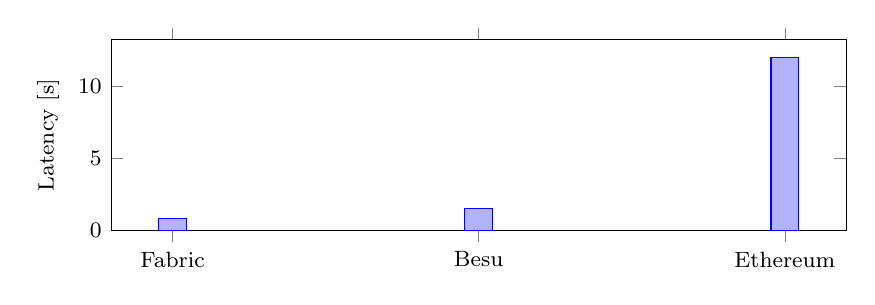
\begin{tikzpicture}
      \begin{axis}[ybar, width=0.9\linewidth, height=40mm, symbolic x coords={Fabric, Besu, Ethereum}, xtick=data, ylabel={Latency [s]}, ymin=0, font=\footnotesize]
        \addplot coordinates {(Fabric,0.8) (Besu,1.5) (Ethereum,12)};
      \end{axis}
    \end{tikzpicture}
    \caption{A pgfplots bar chart.}\label{guide:fig:latex:sub-a}
  \end{subfigure}\hfill
  \begin{subfigure}[b]{0.45\linewidth}
    \centering
    \includegraphics[width=0.6\linewidth]{figures/bme_logo}
    \caption{A PDF image via graphicx.}\label{guide:fig:latex:sub-b}
  \end{subfigure}
  \caption{Subfigures with subcaption.}\label{guide:fig:latex:sub}
\end{figure}

Draw measurement plots from the result files, not from numbers typed into \texttt{coordinates}. Copy the CSV files your benchmark scripts write into \texttt{figures/data/} and read them with \verb|\addplot table[col sep=comma, x=n, y=p95] {figures/data/latency.csv}|. New results then change the figure without editing it by hand. Next to the files, keep a \texttt{README.md} with one row per file: the figure that reads it, the script that wrote it, and the run and code commit it comes from. A reviewer who checks a number against your archived artifact (\cref{guide:chapters:setup}) follows that row. Link the two directions: the paper cites the artifact's tagged release, and the artifact's README names the paper and the result files each of its scripts feeds.

\begin{wrapfigure}{r}{0.3\linewidth}
  \centering
  \captionsetup{format=plain, justification=centering}
  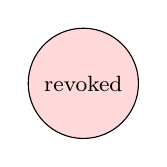
\begin{tikzpicture}
    \node[draw, circle, fill=red!15, minimum size=14mm, font=\footnotesize] {revoked};
  \end{tikzpicture}
  \caption{A wrapped figure.}\label{guide:fig:latex:wrap}
\end{wrapfigure}
Text flows around \cref{guide:fig:latex:wrap}, which wrapfig places at the right margin.
Use wrapfig only for small figures. Do not place it beside a list or section heading, where it breaks.
The paragraph needs enough lines to wrap around the figure, so this example continues for a few sentences.
A revoked credential stays revoked; the registry never forgets.
Verifiers check the registry before accepting a presentation.

\FloatBarrier
The \texttt{\textbackslash FloatBarrier} command from placeins, used above, prevents earlier figures from floating past it.
Use it before a section that must follow all earlier floats.

%----------------------------------------------------------------------------
\section{Coloured boxes (tcolorbox)}\label{guide:latex:boxes}
\begin{infobox}[Information]
  A general-purpose box for background facts.
\end{infobox}
\begin{warnbox}[Threat model caveat]
  A box for warnings and limitations.
\end{warnbox}
\begin{keybox}[Key insight]
  The \texttt{theo} style; any colour works: \texttt{\textbackslash begin\{tcolorbox\}[theo=red, title=...]}.
\end{keybox}

%----------------------------------------------------------------------------
\section{Tables (booktabs, array, tabularx, xltabular, multirow, makecell, rotating)}\label{guide:latex:tables}
\Cref{guide:tab:latex:booktabs} demonstrates booktabs rules and array's \texttt{>\{\textbackslash bfseries\}} for a bold first column. It also uses a stretching tabularx column, multirow, makecell and a coloured row.
\begin{table}[!ht]
  \centering
  \caption{A booktabs table with tabularx, multirow, makecell and a coloured row.}\label{guide:tab:latex:booktabs}
  \begin{tabularx}{\linewidth}{>{\bfseries}l X c}
    \toprule
    Platform & Revocation mechanism & \makecell{Latency\\{[s]}} \\
    \midrule
    \multirow{2}{*}{Fabric} & Chaincode-managed registry & 0.8 \\
     & Private data collections & 1.1 \\
    \rowcolor{gray!15}
    Ethereum & Smart-contract status list & 12 \\
    \bottomrule
  \end{tabularx}
\end{table}

\Cref{guide:tab:latex:long} uses xltabular, which adds page breaks and repeated headers to tabularx.
\begin{xltabular}{\linewidth}{l X}
  \caption{A table that may break across pages.}\label{guide:tab:latex:long}\\
  \toprule
  \textbf{Package} & \textbf{Purpose} \\
  \midrule
  \endfirsthead
  \toprule
  \textbf{Package} & \textbf{Purpose} \\
  \midrule
  \endhead
  todonotes & Visible notes while drafting \\
  glossaries-extra & Abbreviations, notation and terms \\
  tcolorbox & Colored boxes \\
  \bottomrule
\end{xltabular}

\Cref{guide:tab:latex:sideways} has narrow columns under long headings, so rotating's \texttt{sideways} environment turns each heading upright and the columns stay as narrow as their cells. A table too wide even then goes into a \texttt{sidewaystable}, which turns the whole table onto a landscape page of its own; it costs that page however few rows it has.
\begin{table}[!ht]
  \centering
  \caption{Headings turned with rotating, so that narrow columns can carry long headings.}\label{guide:tab:latex:sideways}
  \begin{tabular}{l c c c c c c}
    \toprule
    Approach & \begin{sideways}Offline check\end{sideways} & \begin{sideways}Privacy\end{sideways} & \begin{sideways}Finality\end{sideways} & \begin{sideways}Open source\end{sideways} & \begin{sideways}Throughput\end{sideways} & \begin{sideways}Standardised\end{sideways} \\
    \midrule
    Status list & \gapyes & -- & \gapyes & \gapyes & high & \gapyes \\
    Accumulator & \gapyes & \gapyes & \gapyes & \gappartial & medium & -- \\
    \bottomrule
  \end{tabular}
\end{table}

%----------------------------------------------------------------------------
\section{Algorithms (algorithm, algpseudocode)}\label{guide:latex:alg}
Use \texttt{algorithm} for the captioned float and \texttt{algorithmic} for its steps. \Cref{guide:alg:latex:revoke} shows the notation.
\begin{algorithm}[!ht]
  \caption{Revocation with a freshness check}\label{guide:alg:latex:revoke}
  \begin{algorithmic}[1]
    \Require credential $c$, registry $R$, time $t$
    \If{$c \in R$}
      \State \Return \textsc{already-revoked}
    \EndIf
    \State $R \gets R \cup \{c\}$ \Comment{\cref{guide:eq:latex:fresh}}
    \State \Return \textsc{ok}
  \end{algorithmic}
\end{algorithm}

%----------------------------------------------------------------------------
\section{Code with syntax highlighting (minted, listings)}\label{guide:latex:code}
Use minted, with its Pygments highlighter, for common programming languages.
For a captioned listing, put a \texttt{minted} environment inside a \texttt{listing} float; in running text, use \mintinline{python}{print("inline")}.
Pygments supports over 500 languages. Find lexer names with \texttt{pygmentize -L lexers} or in the documentation's \href{https://pygments.org/docs/lexers/}{lexer list}.
Languages Pygments does not know (Refinery, Tamarin, Lean) go through listings with the styles in \texttt{include/code-languages.tex}: \lstinline[style=lean]{theorem le_succ (n : Nat) : n <= n + 1 := by omega}.
Inline listings must be ASCII under XeLaTeX; Unicode notation such as $\forall$ or $\mathbb{N}$ works in block listings (\cref{lst:latex:lean}).
Both are numbered as listings in one sequence, from \cref{lst:latex:refinery} to \cref{guide:lst:latex:sql}.

\paragraph{Refinery, Tamarin and Lean (listings).}
\Cref{lst:latex:refinery,lst:latex:tamarin,lst:latex:lean} use the listings styles \texttt{refinery}, \texttt{tamarin} and \texttt{lean}.
\begin{lstlisting}[style=refinery, float=tbp, morekeywords={[2]Credential,Issuer,Holder}, caption={Refinery: a credential metamodel with an error predicate.}, label={lst:latex:refinery}]
class Issuer.
class Holder.
class Credential {
    Issuer[1] issuedBy
    Holder[1] heldBy
    contains Credential[0..1] revokes
}

pred selfRevoked(Credential c) <->
    revokes(c, c).

error unissued(Credential c) <->
    !issuedBy(c, _).
\end{lstlisting}

\begin{lstlisting}[style=tamarin, float=tbp, caption={Tamarin: revocation as a multiset-rewriting rule and a lemma.}, label={lst:latex:tamarin}]
theory Revocation
begin
builtins: signing

rule Revoke:
    [ !Issued($I, cred), Fr(~nonce) ]
  --[ Revoked(cred) ]->
    [ !RevokedFact(cred), Out(sign(<cred, ~nonce>, ~sk)) ]

lemma revoked_never_accepted:
  "All cred #i #j. Revoked(cred) @ i & Accepted(cred) @ j ==> j < i"
end
\end{lstlisting}

\begin{lstlisting}[style=lean, float=tbp, caption={Lean 4: the registry only grows (\cref{guide:inv:latex:monotone}).}, label={lst:latex:lean}]
-- A registry is a list of revoked credential identifiers.
def Registry := List Nat

def revoke (r : Registry) (c : Nat) : Registry := c :: r

theorem revoke_monotone (r : Registry) (c x : Nat) :
    x ∈ r → x ∈ revoke r c := by
  intro h
  exact List.mem_cons_of_mem c h
\end{lstlisting}

\FloatBarrier
\paragraph{Common languages (minted).}
\Cref{guide:lst:latex:verify} to \cref{guide:lst:latex:sql} use the Pygments lexers \texttt{python}, \texttt{rust}, \texttt{go}, \texttt{java}, \texttt{typescript}, \texttt{solidity}, \texttt{json}, \texttt{yaml}, \texttt{bash} and \texttt{sql}.
\begin{listing}[!ht]
\begin{minted}{python}
def verify(credential, registry):
    # Reject revoked credentials before checking the signature.
    if credential.id in registry.revoked:
        return False
    return credential.signature_valid()
\end{minted}
\caption{Python.}\label{guide:lst:latex:verify}
\end{listing}

\begin{listing}[!ht]
\begin{minted}{rust}
/// Appends a credential to the registry; revocation is final.
pub fn revoke(registry: &mut HashSet<CredentialId>, id: CredentialId) -> bool {
    registry.insert(id)
}
\end{minted}
\caption{Rust.}\label{guide:lst:latex:rust}
\end{listing}

\begin{listing}[!ht]
\begin{minted}{go}
// IsRevoked reports whether the chaincode state marks the credential as revoked.
func (s *Registry) IsRevoked(ctx contractapi.TransactionContextInterface, id string) (bool, error) {
    v, err := ctx.GetStub().GetState("revoked/" + id)
    return v != nil, err
}
\end{minted}
\caption{Go (a Hyperledger Fabric chaincode function).}\label{guide:lst:latex:go}
\end{listing}

\begin{listing}[!ht]
\begin{minted}{java}
public record Credential(String id, String issuer, Instant expires) {
    public boolean isValidAt(Instant t, Set<String> revoked) {
        return t.isBefore(expires) && !revoked.contains(id);
    }
}
\end{minted}
\caption{Java.}\label{guide:lst:latex:java}
\end{listing}

\begin{listing}[!ht]
\begin{minted}{typescript}
interface StatusEntry { id: string; revoked: boolean }

export async function check(url: string, id: string): Promise<boolean> {
  const list: StatusEntry[] = await (await fetch(url)).json();
  return list.some((e) => e.id === id && e.revoked);
}
\end{minted}
\caption{TypeScript.}\label{guide:lst:latex:ts}
\end{listing}

\begin{listing}[!ht]
\begin{minted}{solidity}
contract RevocationRegistry {
    mapping(bytes32 => bool) public revoked;
    event Revoked(bytes32 indexed id);

    function revoke(bytes32 id) external {
        require(!revoked[id], "already revoked");
        revoked[id] = true;
        emit Revoked(id);
    }
}
\end{minted}
\caption{Solidity.}\label{guide:lst:latex:solidity}
\end{listing}

\FloatBarrier
\begin{listing}[!ht]
\begin{minted}{json}
{
  "@context": ["https://www.w3.org/ns/credentials/v2"],
  "type": ["VerifiableCredential"],
  "issuer": "did:example:university",
  "credentialStatus": { "type": "BitstringStatusListEntry", "statusListIndex": "94567" }
}
\end{minted}
\caption{JSON (a verifiable credential).}\label{guide:lst:latex:json}
\end{listing}

\begin{listing}[!ht]
\begin{minted}{yaml}
# docker-compose.yml: one registry node for the measurements
services:
  registry:
    image: ghcr.io/example/registry:1.4
    ports: ["8080:8080"]
    environment:
      LOG_LEVEL: info
\end{minted}
\caption{YAML.}\label{guide:lst:latex:yaml}
\end{listing}

\begin{listing}[!ht]
\begin{minted}{bash}
#!/usr/bin/env bash
# Run each benchmark size five times and collect the timings.
for n in 10 100 1000 10000; do
  for run in {1..5}; do
    ./bench --credentials "$n" >> "results/$n.csv"
  done
done
\end{minted}
\caption{Bash.}\label{guide:lst:latex:bash}
\end{listing}

\begin{listing}[!ht]
\begin{minted}{sql}
-- Credentials revoked in the last day, per issuer.
SELECT issuer, COUNT(*) AS revoked
FROM revocations
WHERE revoked_at > NOW() - INTERVAL '1 day'
GROUP BY issuer
ORDER BY revoked DESC;
\end{minted}
\caption{SQL.}\label{guide:lst:latex:sql}
\end{listing}
\FloatBarrier

%----------------------------------------------------------------------------
\section{Text (csquotes, ulem, xcolor, xspace, babel, setspace, lineno, comment)}\label{guide:latex:text}
Quotes adapt to the language: \enquote{revocation is final}, and nested: \enquote{the issuer said \enquote{revoked}}.
ulem marks edits: \uline{underlined}, \sout{struck out}, \uwave{wavy}. xcolor colors text: \textcolor{red!70!black}{red}, \colorbox{yellow!40}{highlighted}.
Abbreviation macros use xspace, so they need no trailing braces: \eg the issuer, \ie the registry, Lamport \etal showed.
babel switches the hyphenation and quotes per phrase: \foreignlanguage{magyar}{\enquote{visszavont tanúsítvány}}.

\begin{onehalfspace}
setspace changes the line spacing for a block; this paragraph uses one-and-a-half spacing.
The rest of the thesis is single-spaced, as the TDK rules require.
\end{onehalfspace}

\begin{linenumbers}
lineno numbers lines, so reviewers can point at them.
Wrap a draft paragraph in a \texttt{linenumbers} environment, or put \texttt{\textbackslash linenumbers} in the preamble for the whole document.
\end{linenumbers}

The comment package hides source text without deleting it. The following \texttt{comment} block does not appear in the PDF.
\begin{comment}
This sentence is in the source but not in the PDF.
\end{comment}

%----------------------------------------------------------------------------
\section{Package index}\label{guide:latex:index}
\newcommand{\ctan}[1]{\href{https://ctan.org/pkg/#1}{#1}}
\begin{xltabular}{\linewidth}{>{\ttfamily\raggedright\arraybackslash\hsize=1.1\hsize}X >{\raggedright\arraybackslash\hsize=0.9\hsize}X}
  \caption{Packages loaded by \texttt{include/packages.tex}, with links to examples and CTAN documentation. Open local documentation with \texttt{texdoc <name>}. See also \href{https://tikz.dev/}{tikz.dev} and the \href{https://pgfplots.sourceforge.net/}{pgfplots gallery}.}\label{guide:tab:package-index}\\
  \toprule
  \normalfont\textbf{Package} & \textbf{Shown in} \\
  \midrule
  \endfirsthead
  \toprule
  \normalfont\textbf{Package} & \textbf{Shown in} \\
  \midrule
  \endhead
  \ctan{todonotes} & \cref{guide:latex:todo} \\
  \ctan{glossaries-extra}, \ctan{needspace} & \cref{guide:latex:acro}, and the three lists in the appendix \\
  \ctan{natbib}, \ctan{hyperref}, \ctan{bookmark}, \ctan{orcidlink}, \ctan{fontawesome5} & \cref{guide:latex:cite} \\
  \ctan{cleveref} & \cref{guide:latex:cref}, and every reference in this chapter \\
  \ctan{amsmath}, \ctan{unicode-math} (\ctan{newtx} under pdfLaTeX), \ctan{ntheorem} & \cref{guide:latex:theorems} \\
  \ctan{enumitem} & \cref{guide:latex:tags} \\
  \ctan{graphicx}, \ctan{svg}, \ctan{tikz}, \ctan{pgfplots} (with its \texttt{groupplots} library), \ctan{subcaption}, \ctan{wrapfig}, \ctan{placeins} & \cref{guide:latex:figures}; \texttt{groupplots} in \cref{guide:fig:caption-example} \\
  \ctan{forest} & \cref{guide:fig:mindmap}, the skeleton mind map \\
  \ctan{tcolorbox} & \cref{guide:latex:boxes} \\
  \ctan{booktabs}, \ctan{array}, \ctan{tabularx}, \ctan{xltabular}, \ctan{multirow}, \ctan{makecell}, \ctan{rotating} & \cref{guide:latex:tables} \\
  \ctan{algorithms}, \ctan{algorithmicx} & \cref{guide:latex:alg} \\
  \ctan{listings}, \ctan{minted} & \cref{guide:latex:code} \\
  \ctan{csquotes}, \ctan{ulem}, \ctan{xcolor}, \ctan{xspace}, \ctan{babel}, \ctan{setspace}, \ctan{lineno}, \ctan{comment} & \cref{guide:latex:text} \\
  \ctan{caption} & Every caption: bold labels, hanging indent \\
  \ctan{anysize} & Page margins, set with \texttt{\textbackslash marginsize} in \texttt{thesis.tex} \\
  \ctan{microtype} & Character protrusion and font expansion on every page \\
  \ctan{emptypage} & Blank pages before chapters have no page number \\
  \ctan{ifxetex}, \ctan{ifluatex}, \ctan{fontspec}, \ctan{fontenc}, \ctan{inputenc}, \ctan{lm}, \ctan{newtx} & Text in TeX Gyre Termes (Times), code in Latin Modern Mono, under XeLaTeX, LuaLaTeX and pdfLaTeX \\
  \bottomrule
\end{xltabular}
